\section{Assessment}
\label{sec:assessment}
\subsection{Experimental Setup}
We implement our PCDNet in PyTorch \cite{paszke2019pytorch} and train it for 300 epochs with the batch size of 32 on two NVIDIA GeForce RTX 3090 GPUs. We use stochastic gradient descent (SGD) \cite{amari1993backpropagation} with a momentum of 0.937 and a weight decay of $5 \times 10 ^{-4}$ during training. The initial learning rate is set to 0.01 and decayed to 0.001 using a cosine annealing schedule. We initialize PCDNet randomly and load the weights of CSPDarknet53 \cite{wang2020cspnet} pre-trained on ImageNet \cite{imagenet_cvpr09} for the encoder part. To increase the diversity and complexity of the training samples, we apply data augmentations including random cropping, random flipping, and mosaic \cite{redmon2018yolov3}. We use the evaluation metrics of Microsoft COCO \cite{lin2014microsoft} for validation.

\begin{table}[ht]
\caption{Quantitative comparison against state-of-the-art polarization-based detectors ($\star$), single-stage detectors ($\dag$), two-stage detectors ($\ddag$), anchor-based detectors ($\triangle$), anchor-free detectors ($\circ$), and self-supervised method ($\S$).}
\small
\centering
\renewcommand\arraystretch{0.9}
\setlength{\tabcolsep}{2.6pt}
\begin{tabular}{lccccc}
\hline\hline
Methods	&	Pub'Year	&	Backbone	&	AP	&	AP50	&	AP75	\\
\hline
Faster R-CNN$^{\ddag\triangle}$ 	&	NeurIPS'15	&	Res50	&	44.8	&	75.4	&	45.4	\\
SSD$^{\dag\circ}$ 	&	ECCV'16	&	VGG16	&	25.5	&	52.6	&	22.6	\\
Cascade R-CNN$^{\ddag\triangle}$ 	&	CVPR'18	&	Res50	&	45.8	&	73.2	&	47.8	\\
CornerNet$^{\dag\circ}$ 	&	ECCV'18	&	Res50	&	19.8	&	47.4	&	29.6	\\
P-SSD I$^{\star\dag\circ}$ 	&	ITSC'19	&	VGG16	&	25.9 	&	53.1	&	22.7	\\
P-SSD S$^{\star\dag\circ}$ 	&	ITSC'19	&	VGG16	&	23.0 	&	48.9	&	20.1	\\
FCOS$^{\dag\circ}$ 	&	ICCV'19	&	Res50	&	23.1	&	50.9	&	18.4	\\
DH R-CNN$^{\ddag\triangle}$ 	&	CVPR'20	&	Res50	&	32.7	&	65.3	&	28.2	\\
Dynamic R-CNN$^{\ddag\triangle}$ 	&	ECCV'20	&	Res50	&	46.2	&	74.2	&	48.0	\\
EfficientDet$^{\ddag\triangle}$ 	&	CVPR'20	&	D3	&	45.3	&	73.0	&	46.3	\\
VarifocalNet$^{\dag\circ}$  & CVPR'21 & Res50 & 44.2 &	73.5 &	44.4	\\
D-DETR$^{\dag\circ}$ 	&	ICLR'21	&	Res50	&	43.8	&	74.9	&	44.3	\\
DDOD$^{\dag\circ}$ 	&	MM'21	&	Res50	&	43.5	&	73.0	&	43.3	\\
TOOD$^{\dag\triangle}$ 	&	ICCV'21	&	Res50	&	44.3	&	74.3	&	44.6	\\
YOLOX$^{\dag\circ}$ 	&	arXiv'21	&	YOLOX-l	&	54.3	&	82.5	&	56.7	\\
YOLOv7$^{\dag\triangle}$	&	arXiv'22	&	Dark53	&	57.6	&	84.3	&	60.3	\\
RTMDet$^{\dag\circ}$ 	&	arXiv'22	&	RTMDet-l	&	53.9	&	81.4	&	56.7	\\
DINO$^{\dag\circ\S}$ 	&	ICLR'22	&	Res50	&	52.7	&	81.8	&	54.8	\\
YOLOv8$^{\dag\circ}$ 	&	-'23	&	YOLOv8-l	&	56.8	&	83.6	&	59.0	\\
\hline
\textbf{PCDNet$^\star$}	&	\textbf{Ours}	&	Dark53	&	\textbf{58.5}	&	\textbf{85.2}	&	\textbf{61.5}	\\
\hline\hline
\end{tabular}
\label{tab:comparison}
\end{table}

\begin{figure*}[htp]
    \centering
    \begin{center}
        % \includegraphics[width=\linewidth]{figure/comparison.pdf}
        \includegraphics[width=\linewidth,height=10.5cm]{figure/comparison.pdf}
    \end{center}
    \caption{Qualitative comparison of PCDNet against state-of-the-art detectors retrained on RGB-P Car dataset.} 
    \label{fig:comparison}
\end{figure*}

\subsection{Qualitative and Quantitative Evaluation}
We extensively compare our PCDNet with 19 state-of-the-art methods by retraining and testing all methods on the RGB-P Car dataset using their original settings. The compared methods include two-stage detectors such as EfficientDet \cite{tan2020efficientdet} and the R-CNN family \cite{Ren_2017, Cai_2019, zhang2020dynamic}, and one-stage detectors such as SSD \cite{liu2016ssd}, and YOLO family \cite{ge2021yolox, wang2022yolov7, ultralytics2023yolov8}. These methods also comprise anchor-based methods such as the R-CNN family and YOLOv7 \cite{wang2022yolov7}, and anchor-free methods such as CornerNet \cite{law2018cornernet}, VarifocalNet \cite{zhang2021varifocalnet}, and YOLOv8 \cite{ultralytics2023yolov8}. Some detectors use traditional convolutional networks such as FCOS \cite{tian2019fcos} and RTMDet \cite{lyu2022rtmdet} while others use transformer structures, such as DeformableDETR \cite{zhu2020deformable} and DINO \cite{zhang2022dino} that employs self-supervised learning. We also include the P-SSD \cite{blin2019road} that utilizes polarization information. The quantitative evaluation results are reported in Tab. \ref{tab:comparison}. We can see that our method outperforms all competing state-of-the-art methods. 

Fig. \ref{fig:comparison} further qualitatively demonstrates the benefits of our method: a) in poorly lit indoor parking lots, distinguishing black cars behind pillars is extremely challenging (the first two rows). The compared methods tend to conflate the shadow and the black car (\textit{i.e.}, merging cars on either side of the pillar into a single entity or treating partial views of the car as one object) while our PCDNet can handle such ambiguities; b) in the third example, all methods except our PCDNet fail to detect a partially visible car obstructed by another car or misplace it with the previous car; c) in the fourth example, RGB-based methods wrongly identify distant pedestrians as cars, but our PCDNet method can effectively eliminate such interference with the help of polarization cues; d) the fifth and sixth examples depict black cars in an outdoor parking lot at night which are very hard to be distinguished in the RGB image. Despite the enhancement through ZeroDCE \cite{guo2020zero}, the sixth example remains unclear. By contrast, polarization imaging is robust to low light conditions, enabling our robust car detector PCDNet; and e) the last row shows a virtual car reflected in a mirror located at the upper-left corner of the image. The mirrored virtual car and the rest of the mirror regions exhibit similar and smooth AoLP, providing useful cues for PCDNet to recognize this region as background. 


\subsection{Ablation Study}
\textbf{Impact of Spectral Intensity and Polarization Cues.} We conduct a series of ablation experiments to demonstrate the effects of spectral intensity and polarization cues on car detection (Tab. \ref{tab:abl_input}).
The results show that: a) combining different forms of polarization cues with RGB as the input of PCDNet can improve the car detection accuracy (\textit{C}, \textit{D}, \textit{F}, \textit{G}, \textit{K} and \textit{L} are higher than \textit{B}); b) DoLP cues have a greater impact than AoLP cues (\textit{D}, \textit{J} and \textit{L} are better than \textit{C}, \textit{I} and \textit{K}, respectively); c) stacking AoLP and DoLP on RGB in the channel dimension does not boost performance (\textit{E} is slightly lower than \textit{B}), possibly because the characteristic gap between different modalities hinders effective features extraction; d) spectral intensity and polarization are more beneficial than monochromatic intensity and polarization for car detection (comparing paired \textit{B} and \textit{H}, \textit{C} and \textit{K}, \textit{D} and \textit{L}, \textit{I} and \textit{K}, \textit{J} and \textit{L}); e) enhancing RGB image via ZeroDCE \cite{guo2020zero} is less effective than introducing polarization (\textit{M} performs worse than \textit{C}-\textit{G}, \textit{K} and \textit{L}).
Fig. \ref{fig:abl_input} provides visual support for these observations.

\begin{table}[t]
\small
\centering
\caption{Quantitative comparisons of ablation with different inputs. ``stacked I'' denotes the stacked intensity measurements with a linear polarization angle of 0$^{\circ}$, 45$^{\circ}$ and 135$^{\circ}$ and ``stacked S'' refers to the stacked Stokes elements S0, S1 and S2 \cite{blin2019road}.}
\begin{tabular}{clccc}
\hline\hline
	&	PCDNet Input	&	AP	&	AP50	&	AP75	\\
 \hline
\textit{A}	&	RGB, AoLP and DoLP (original)	&	58.5 	&	85.2 	&	61.5 	\\
\hline
\textit{B}	&	RGB only	&	57.6 	&	84.3 	&	60.2 	\\
\textit{C}	&	RGB and AoLP	&	58.0 	&	84.6 	&	60.7 	\\
\textit{D}	&	RGB and DoLP	&	58.3 	&	85.4 	&	61.1 	\\
\textit{E}	&	stacked RGB, AoLP and DoLP	&	57.5 	&	84.3 	&	59.9 	\\
\textit{F}	&	RGB and stacked I	&	58.0 	&	84.1 	&	61.0 	\\
\textit{G}	&	RGB and stacked S	&	57.8 	&	84.8 	&	60.4 	\\
\textit{H}	&	Gray only	&	57.4 	&	84.3 	&	60.0 	\\
\textit{I}  &   Gray and mono AoLP & 57.5 & 84.5 & 60.5 \\
\textit{J}  &   Gray and mono DoLP & 57.6 & 84.9 & 60.1 \\
\textit{K}	&	RGB and mono AoLP	&	57.9 	&	84.6 	&	60.5 	\\
\textit{L}	&	RGB and mono DoLP	&	58.2 	&	84.9 	&	60.6 	\\
\textit{M}  &   Enhanced RGB & 57.4 & 84.0 & 60.0 \\
\hline\hline
\end{tabular}
\label{tab:abl_input}
\end{table}

\begin{figure}[t]
    \centering
    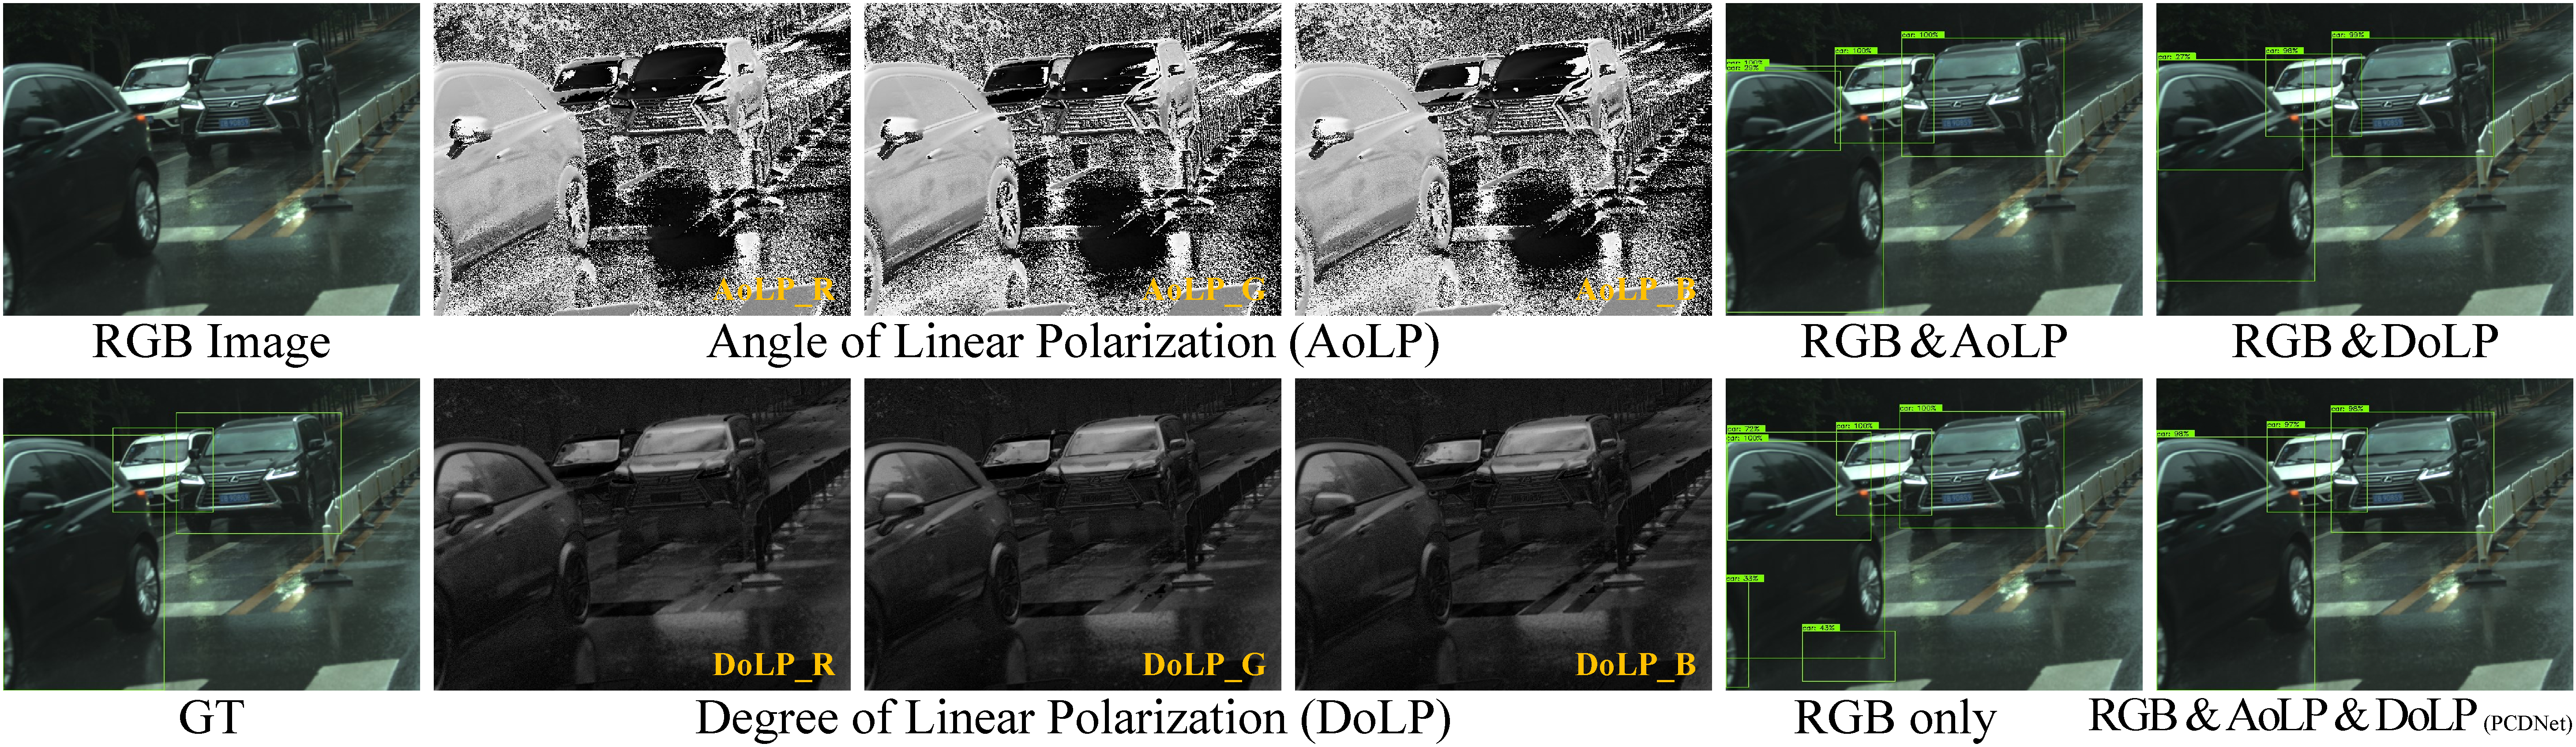
\includegraphics[width=1\linewidth]{figure/abl_input.pdf}
    \caption{Qualitative comparison of ablation with different inputs. The model with RGB intensity only is susceptible to interference from ghost car caused by water on the road.}
    \label{fig:abl_input}
\end{figure}

\textbf{Influence of PCDNet Components.}
First, we investigate the performance of different strategies for fusing AoLP and DoLP inputs. From Tab. \ref{tab:abl_module}(\textit{A}-\textit{D}), we observe that our PI module is more effective than the simple fusion methods including concatenation, addition and element-wise multiplication.
Second, by removing MP module \ref{tab:abl_module}(\textit{E}) from the original PCDNet (A), the detection performance declines. This demonstrates that exploring the polarized material features of cars across all learning samples is useful. We also explore the influence of applying MSP and MCP on different levels of features. The results in Tab. \ref{tab:abl_module}(\textit{A},\textit{F}-\textit{G}) show that applying MSP on shallower features and MCP on deeper features can yield better performance.
Finally, we validate the effectiveness of CDDQ module.
Removing the CDDQ module (\textit{I}) from PCDNet (\textit{A}), which causes the feature extraction processes of the RGB and polarization to be independent from each other, leads to the performance drop. We also demonstrate the benefits of the CWDA and SDMD in the CDDQ module by removing either of them (\textit{J} and \textit{K}). 

\begin{table}[t]
\small
\centering
\caption{Quantitative comparisons of ablation with different modules demonstrate that all component of PCDNet contributes to the overall performance. We used sequences of three letters separated by '-' and enclosed in parentheses to represent different combinations of MSP and MCP.}
\begin{tabular}{clccc}
\hline\hline
	&	Ablation	&	AP	&	AP50	&	AP75	\\
 \hline
\textit{A}	&	PCDNet (original)	&	58.5 	&	85.2 	&	61.5 	\\
\hline
\textit{B}	&	Input RGB and [AoLP DoLP]	&	58.2 	&	85.4 	&	60.9 	\\
\textit{C}	&	Input RGB and AoLP+DoLP	&	58.1 	&	84.8 	&	60.5 	\\
\textit{D}	&	Input RGB and AoLP*DoLP	&	58.1 	&	84.8 	&	60.5 	\\
\hline
\textit{E}	&	A \textit{w/o} MP	&	56.9 	&	84.2 	&	59.2 	\\
\textit{F}	&	A \textit{w/} M(S-S-S)P	&	58.2 	&	85.2 	&	60.8 	\\
\textit{G}	&	A \textit{w/} M(S-C-C)P	&	58.2 	&	85.0 	&	60.9 	\\
\textit{H}	&	A \textit{w/} M(C-C-C)P	&	58.1 	&	85.0 	&	61.1 	\\
\hline
\textit{I}	&	A \textit{w/o} CDDQ	&	58.0 	&	84.7 	&	60.8 	\\
\textit{J}	&	A \textit{w/o} SDMD	&	58.2 	&	85.2 	&	60.8 	\\
\textit{K}	&	A \textit{w/o} CWDA	&	58.3 	&	85.1 	&	61.1 	\\
\hline\hline
\end{tabular}
\label{tab:abl_module}
\end{table}

\subsection{Limitations}

When both the RGB intensity and the polarization measurement yield weak car signals, our method's effectiveness declines. Specifically, in low-light scenarios, when a car approaches on an unlit road, the strong light from its headlights can create a ``hole'' in both the RGB and polarization and obscure the entire car. We illustrate such an example in Fig. \ref{fig:failure} where the extreme HDR and heavy motion blur in the captured image limit its depiction of both RGB and polarization. In these challenging scenarios, prior RGB-based methods and even human vision are powerless.

\begin{figure}[t]
    \centering
    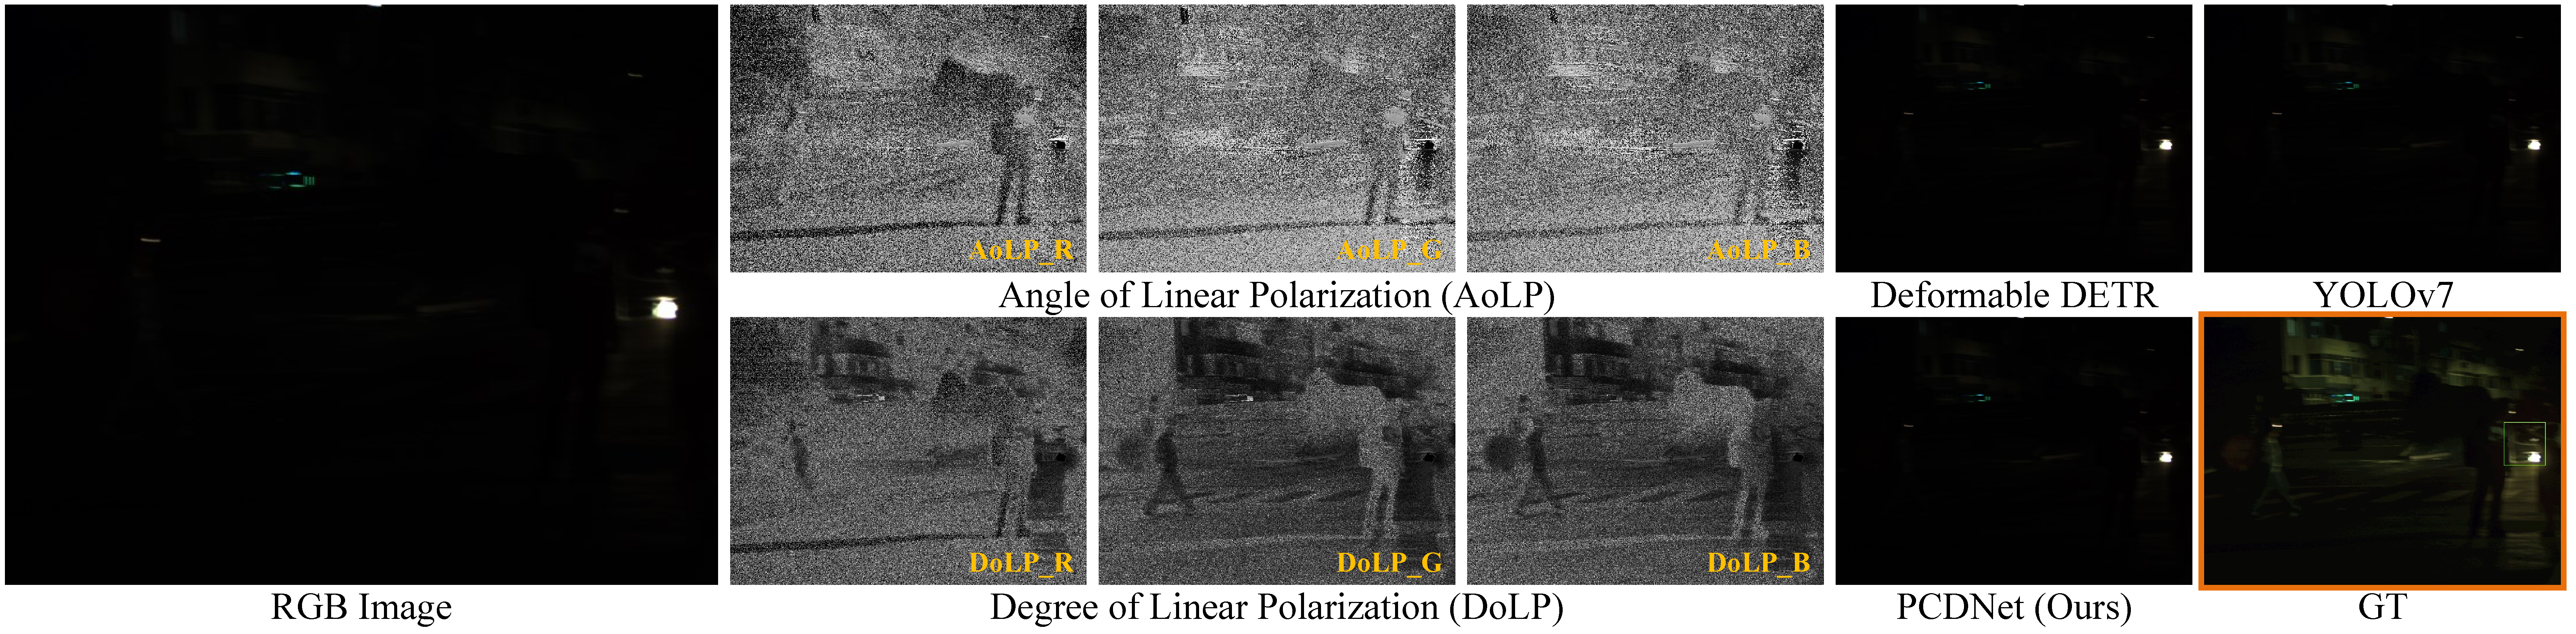
\includegraphics[width=1\linewidth]{figure/failure.pdf}
    \caption{PCDNet has limited ability to handle extreme HDR or heavy motion blur cases.}
    \label{fig:failure}
\end{figure}
